% !TEX root = report.tex
\documentclass[letterpaper,12pt]{article}
\usepackage{tabularx} % extra features for tabular environment
\usepackage{amsfonts}
\usepackage{amsmath}  % improve math presentation
\usepackage{amssymb}
\usepackage{graphicx} % takes care of graphic including machinery
\usepackage[margin=1in,letterpaper]{geometry} % decreases margins
\usepackage{cite} % takes care of citations
\usepackage[final]{hyperref} % adds hyper links inside the generated pdf file
\usepackage{multicol}
\usepackage{enumitem}
\usepackage{mwe}
\setlength{\columnsep}{1cm}
\hypersetup{
        colorlinks=true,       % false: boxed links; true: colored links
        linkcolor=blue,        % color of internal links
        citecolor=blue,        % color of links to bibliography
        filecolor=magenta,     % color of file links
        urlcolor=blue         
}
%++++++++++++++++++++++++++++++++++++++++


\begin{document}

\title{\textbf{Super-Resolution using Deep Learning} \\ CSC420H1: Project Report (CosmicMangos)}


\author{Michal Fishkin (1004817219) \\ Siddhant Jain (1004070024) \\ Robert Wu (1004256798)}

\maketitle

\section*{Abstract}
Images with higher resolutions capture and preserve more details, and are usually easier to work with. While data and information are valuable, so are bandwidth and storage. Sometimes images are of lower resolution than we'd like, like in photographs taken by low-resolution cameras and compressed images that are more suitable for fast data transfer. Benefits of lower resolutions include higher framerates, lower latency and less expensive storage. Unfortunately, as a natural consequence, these lower-resolution images almost always contain less information than their higher-resolution counterparts.

\section*{Introduction}

In order to work with more information, it's useful to produce an image with higher resolution, what we refer to as ``super-resolution" (SR). This task allows you to extract more information than was in the original images and hopefully produce a more pleasant image to the human eye. However, this problem is ill-posed. An ill-posed problem is defined as one that violates one of the following properties.

\begin{enumerate}
    \item A solution exists;
    \item The solution is unique;
    \item The solution changes smoothly with initial conditions.
\end{enumerate}

As super-resolution is about synthesizing pixels and details that don't exist in the original images, we can assume that in general, the second property is violated. Thus the various solutions to the problem will have their own ways of ``predicting" or ``generating" the synthetic pixels. They can employ local generation, such as interpolation and image pyramids, or even deep learning, which can identify larger patterns and contexts from training examples to make better predictions.

\pagebreak

\section*{Literature Review}

To begin, we'll mention some simple classical methods used to solve this problem. These are methods introduced in our lectures in CSC420, and they helped us develop an intuition for the SR problem.

\begin{itemize}
    \item Copying existing pixels.
    \item Image filters.
    \item Interpolation (linear interpolation in particular).
    \item Image Pyramids
\end{itemize}

\begin{figure}[h!]
    \centering
    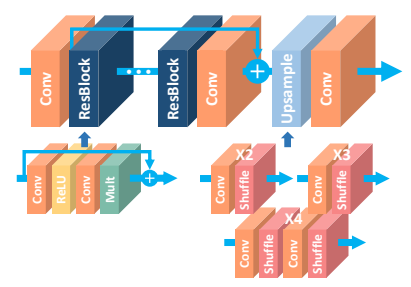
\includegraphics[scale=.7]{opencv_/architecture.png}
    \caption{Enhanced Deep Super-Resolution Network (EDSRN). \cite{Lim2017}}
\end{figure}

Of course, to produce an SR image, classical methods have access only to the pixels in the original image. This limitation could be overcome using previous ``learned" context, as the last majority of images that we work with will have similar patterns to other images. As there is an extensive amount of work in this field, we have reviewed some of the deep learning algorithms proposed in the recent literature. 

\begin{itemize}
    \item Super-resolution through neighbor embedding, \cite{HKUST} a novel method for solving single-image super-resolution problems, inspired by locally linear embedding (LLE). This early solution leverages training examples to provide local geometry of the manifolds formed from patches taken from low and high resolution images. \cite{HKUST}
    \item A Fully Progressive Approach to Single-Image Super-Resolution. \cite{DisneyResearch} The proposed method uses a progressive (from easy to hard) learning process aided by Generative Adversarial Networks (GANs). Interestingly, the authors reduce memory usage and training time while still increasing accuracy, with the use of an asymmetric architecture of Dense Compression Units (DCUs). \cite{DisneyResearch}
    \item Deep Learning for Single Image Super-Resolution: A Brief Review. \cite{DLSISR} This is a review paper of the existing solutions to SISR, and we can evaluate them in choosing algorithms and considering caveats. While we didn't quite use the implementations presented in this publication, we took as insight the challenges the authors faced:  ``the  acceleration  of  deep models, the extensive comprehension of deep models and thecriteria  for  designing  and  evaluating  the  objective  functions." \cite{DisneyResearch}
    \item Neural-Enhance, \cite{AlexJC} a deep learning implementation using extensive neural networks that "hallucinate" details of images. This relies on \href{https://github.com/Lasagne/Lasagne}{Lasagne}, using Theano to support Convolutional Neural Networks (CNNs) and Long Short-Term Memory (LSTM). \cite{Lasagne} Based on the author's descriptions, we hypothesize this solution might be rather sensitive to noise.
    \item Enhanced Deep Super-Resolution Network (EDSRN). \cite{Lim2017} A residual network without unnecessary modules and progressively expanding model sizes in training. The authors propose a ``new multi-scale deep super-resolution system (MDSR) and training method,which  can  reconstruct  high-resolution  images  of  differentupscaling factors in a single model." \cite{Lim2017}
    \item Image Super-Resolution using Convolution Neural Networks and Autoencoders\\(CNNs+Autoencoders). \cite{PatelH}. This tutorial demonstrates how to combine CNNs and Autoencoders to generatively predict and enhance images. \cite{PatelH} This solution was appealing because it's quite explicit about its architecture and provides easy ways to tune the hyperparameters and adjust the structure.
\end{itemize}

Because deep learning is computationally expensive, we will test and evaluate the most promising methods that are feasible to implement. We will consider EDSRN, Neural-Enhance, and CNNs+Autoencoders to measure their results against classical methods.

\pagebreak
\section*{Methodology, Experiments, Results}

\begin{figure*}[h!]
    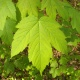
\includegraphics[width=.2\textwidth]{small-test-set_processed/green-maple-leaf.jpg}\hfill
    
\includegraphics[width=.2\textwidth]{small-test-set_processed/home-office.jpg}\hfill
    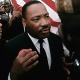
\includegraphics[width=.2\textwidth]{small-test-set_processed/martin-luther-king.jpg}\hfill
    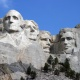
\includegraphics[width=.2\textwidth]{small-test-set_processed/mount-rushmore.jpg}\hfill
    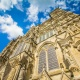
\includegraphics[width=.2\textwidth]{small-test-set_processed/salisbury-cathedral.jpg}
    \caption{Preprocessed images ($80\times80$).}
\end{figure*}

\begin{figure*}[h!]
    
\includegraphics[width=.2\textwidth]{small-test-set_reduced/green-maple-leaf.jpg}\hfill
    
\includegraphics[width=.2\textwidth]{small-test-set_reduced/home-office.jpg}\hfill
    
\includegraphics[width=.2\textwidth]{small-test-set_reduced/martin-luther-king.jpg}\hfill
    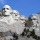
\includegraphics[width=.2\textwidth]{small-test-set_reduced/mount-rushmore.jpg}\hfill
    
\includegraphics[width=.2\textwidth]{small-test-set_reduced/salisbury-cathedral.jpg}
    \caption{Reduced images ($40\times40$).}
\end{figure*}

For evaluation, we chose a small but varied test set of five images, each unique in same aspect. See the \texttt{small-test-set} folder in our repository for the originals.

\begin{itemize}
    \item \textbf{Green Maple Leaf}: Small details of close-up object.
    \item \textbf{Home Office}: Many objects in one setting.
    \item \textbf{Martin Luther King Jr.}: A person's face and body language.
    \item \textbf{Mount Rushmore}: Details of far objects.
    \item \textbf{Salisbury Cathedral}: Upward angle at a façade.
\end{itemize}

In order to evaluate the methods on the same standards, we chose $80\times80$ as the base resolution, and $40\times40$ as the reduced resolution. As the original images had a variety of resolutions, we had to resize them down and ``centre-crop" them (cropping the largest centre-square) using \texttt{preprocessing/preprocessed.py} [Figure 2]. Then, to produce the reduced resolution images, we used \href{https://medium.com/@wenrudong/what-is-opencvs-inter-area-actually-doing-282a626a09b3}{\texttt{cv2.INTER\_AREA}} \cite{DongW} in \texttt{preprocessing/reduce.py} to produce our $40\times40$ images [Figure 3].

\pagebreak

We will use the four methods to generate SR images from the reduced test set, that are $80\times80$. These dimensions are chosen because we will compare the resulting SR images to the original images to evaluate how well each method predicts/generates the missing pixels.

\begin{figure*}[h!]
    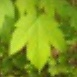
\includegraphics[width=.2\textwidth]{linear/green-maple-leaf.jpg}\hfill
    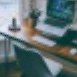
\includegraphics[width=.2\textwidth]{linear/home-office.jpg}\hfill
    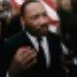
\includegraphics[width=.2\textwidth]{linear/martin-luther-king.jpg}\hfill
    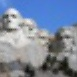
\includegraphics[width=.2\textwidth]{linear/mount-rushmore.jpg}\hfill
    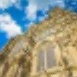
\includegraphics[width=.2\textwidth]{linear/salisbury-cathedral.jpg}
    \caption{Super-resolution using linear interpolation.}
\end{figure*}

\begin{figure*}[h!]
    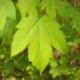
\includegraphics[width=.2\textwidth]{opencv_/green-maple-leaf.jpg}\hfill
    
\includegraphics[width=.2\textwidth]{opencv_/home-office.jpg}\hfill
    
\includegraphics[width=.2\textwidth]{opencv_/martin-luther-king.jpg}\hfill
    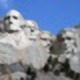
\includegraphics[width=.2\textwidth]{opencv_/mount-rushmore.jpg}\hfill
    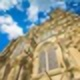
\includegraphics[width=.2\textwidth]{opencv_/salisbury-cathedral.jpg}
    \caption{Super-resolution using EDSRN.}
\end{figure*}

Our linear interpolation method was implemented in \texttt{linear\_inter.ipynb} and run on all the images to produce the SR images seen in [Figure 4]. In \texttt{linear\_inter.ipynb}, we also employed EDSRN to produce images in [Figure 5]. \\

\begin{figure*}[h!]
    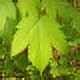
\includegraphics[width=.2\textwidth]{alexjc_neural-enhance/green-maple-leaf.jpg}\hfill
    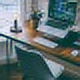
\includegraphics[width=.2\textwidth]{alexjc_neural-enhance/home-office.jpg}\hfill
    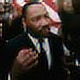
\includegraphics[width=.2\textwidth]{alexjc_neural-enhance/martin-luther-king.jpg}\hfill
    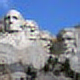
\includegraphics[width=.2\textwidth]{alexjc_neural-enhance/mount-rushmore.jpg}\hfill
    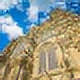
\includegraphics[width=.2\textwidth]{alexjc_neural-enhance/salisbury-cathedral.jpg}
    \caption{Super-resolution using Neural-Enhance.}
\end{figure*}

Using the existing implementation of Neural Enhance\cite{AlexJC}, deployed to a dockerized container on Google Compute Platform we generated the SR images in [Figure 6]. Neural Enhance provides pre-trained models of a purely CNN nature. Neural Enhance contains 16 Convolution layers and 4 max-pooling layers.

\pagebreak

\begin{figure*}[h!]
    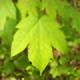
\includegraphics[width=.2\textwidth]{cnn-autoencoders/green-maple-leaf.jpg}\hfill
    
\includegraphics[width=.2\textwidth]{cnn-autoencoders/home-office.jpg}\hfill
    
\includegraphics[width=.2\textwidth]{cnn-autoencoders/martin-luther-king.jpg}\hfill
    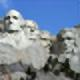
\includegraphics[width=.2\textwidth]{cnn-autoencoders/mount-rushmore.jpg}\hfill
    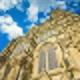
\includegraphics[width=.2\textwidth]{cnn-autoencoders/salisbury-cathedral.jpg}
    \caption{Super-resolution using CNNs and Autoencoders.}
\end{figure*}

And finally, in using CNNs and Autoencoders, we followed a \href{https://towardsdatascience.com/image-super-resolution-using-convolution-neural-networks-and-auto-encoders-28c9eceadf90}{Towards Data Science tutorial} \cite{PatelH} and trained the model on the ``Labeled Faces in the Wild" dataset \cite{LFWTech} \cite{LFWTechUpdate} using a $5$\% partition and maximum of $100$ epochs. For this method, we adjusted the hyperparameters, and cleaned the validation set with minor data processing and adding our test images. Furthermore, we added a normalizing function \texttt{normalize()} as the produced images had scaling that slightly exceeded the upper bounds of pixel values. Using $50$\% pixalating (roughly equivalent to our downsampling preprocessing reduction), the cost function reached converged at the plateau in $51$ epochs, when our final results were produced [Figure 7].

\subsection*{Evaluation}

In measuring the quality of the super-resolution (SR) outputs numerically, we used the following metrics, the latter two of which we devised to be creative.

\begin{enumerate}
    \item Mean Squared-Error (MSE): Mean pixel-by-pixel squared differences between the original image and the SR output. Implemented in \texttt{mse.py}.
    \item Mean Squared-Gradient-Errors (MSGE): Mean pixel-by-pixel squared gradient (computed using Sobel) differences between the original image and the SR output. \textit{The values are expressed as pairwise gradient components $(G_x, G_y$).} Implemented in \texttt{MSGE.py}.
    \item Corner Detection (Count): (SR Corner Count - Original Corner Count). This metric is a real number for each single method/image pair, and should be interpreted by \textit{magnitude}. Implemented in \texttt{corner-detection.py}.
    \item Corner Detection (Nearest Corner Distance): $(D_{OtoSR},D_{SRtoO})$ where $D_{OtoSR}$ is defined as the average distance between corners in the original images and their closest neighbour pixel in the SR image and $D_{SRtoO}$ is defined as the average distance between corners in the SR images and their closest neighbour pixel in the original image. This is roughly equivalent to the effect of Corner Matching as we're finding the nearest corners of another image with the same perspective.
\end{enumerate}

\pagebreak
\subsubsection*{Results}

\begin{center}\begin{tabular}{ |c||c|c|c|c| }
    \hline
    \multicolumn{5}{|c|}{Green Maple Leaf Results} \\
    \hline
    & MSE & MSGE\* & Corner Count & Nearest-Corner\\
    \hline
    Linear Interpolation & $61.52$ & $(274982, 222540)$ & $-524$ & $(1.375, 0.412)$\\
    EDSRN & $55.04$ & $(31710, 26342)$ & $-216$ & $(0.850, 0.570)$\\
    Neural-Enhance & $187.30$ & $(47674, 35089)$ & $-308$ & $(0.814, 0.412)$\\
    CNNs+Autoencoders & $84.54$ & $(31374, 20961)$ & $-177$ & $(0.796, 0.572)$\\
    \hline
\end{tabular}\end{center}

\begin{center}\begin{tabular}{ |c||c|c|c|c| }
    \hline
    \multicolumn{5}{|c|}{Home Office Results} \\
    \hline
    & MSE & MSGE\* & Corner Count & Nearest-Corner\\
    \hline
    Linear Interpolation & $72.01$ & $(330256, 419536)$ & $87$ & $(0.453, 0.614)$\\
    EDSRN & $62.65$ & $(39649, 51109)$ & $-199$ & $(0.500, 0.268)$\\
    Neural-Enhance & $334.57$ & $(74994, 74682)$ & $-86$ & $(0.709, 0.464)$\\
    CNNs+Autoencoders & $62.43$ & $(31148, 37969)$ & $-2$ & $(0.494, 0.594)$\\
    \hline
\end{tabular}\end{center}

\begin{center}\begin{tabular}{ |c||c|c|c|c| }
    \hline
    \multicolumn{5}{|c|}{Martin Luther King Jr. Results} \\
    \hline
    & MSE & MSGE\* & Corner Count & Nearest-Corner\\
    \hline
    Linear Interpolation & $52.20$ & $(574745, 433759)$ & $7$ & $(0.816, 0.700)$\\
    EDSRN & $42.21$ & $(53709, 36984)$ & $59$ & $(0.663, 0.713)$\\
    Neural-Enhance & $259.24$ & $(87961, 61993)$ & $46$ & $(0.604, 0.660)$\\
    CNNs+Autoencoders & $43.17$ & $(34841, 25462)$ & $-27$ & $(0.762, 0.656)$\\
    \hline
\end{tabular}\end{center}

\begin{center}\begin{tabular}{ |c||c|c|c|c| }
    \hline
    \multicolumn{5}{|c|}{Mount Rushmore Results} \\
    \hline
    & MSE & MSGE\* & Corner Count & Nearest-Corner\\
    \hline
    Linear Interpolation & $59.88$ & $(312489, 377194)$ & $179$ & $(0.674, 0.822)$\\
    EDSRN & $53.06$ & $(38247, 45897)$ & $-201$ & $(0.809, 0.540)$\\
    Neural-Enhance & $197.42$ & $(43156, 59944)$ & $-30$ & $(0.774, 0.653)$\\
    CNNs+Autoencoders & $53.36$ & $(30383, 38007)$ & $-253$ & $(0.878, 0.495)$\\
    \hline
\end{tabular}\end{center}

\begin{center}\begin{tabular}{ |c||c|c|c|c| }
    \hline
    \multicolumn{5}{|c|}{Salisbury Cathedral Results} \\
    \hline
    & MSE & MSGE\* & Corner Count & Nearest-Corner\\
    \hline
    Linear Interpolation & $86.20$ & $(438483, 437998)$ & $-543$ & $(0.617, 0.444)$\\
    EDSRN & $79.80$ & $(67422, 65934)$ & $-276$ & $(0.580, 0.490)$\\
    Neural-Enhance & $414.76$ & $(89386, 91589)$ & $-293$ & $(0.557, 0.462)$\\
    CNNs+Autoencoders & $80.17$ & $(52132, 55888)$ & $-420$ & $(0.590, 0.459)$\\
    \hline
\end{tabular}\end{center}


\pagebreak
\section*{Conclusion}

After reviewing the results, we made the following observations.

\begin{itemize}
    \item In Mean Squared-Error (MSE), Neural-Enhance was consistently the worst-performing method. This is likely due to the noise that Neural-Enhance generates everywhere on every image.
    \item With the exception of the Green Maple Leaf, CNNs and Autoencoders performed achieved the best MSE results or a very close second-best.
    \item Linear interpolation performed very poorly in the mean squared-gradient-errors. For some reason the errors are in six figures.
    \item Meanwhile, CNNs and Autoencoders performed well in this respect, with the lowest squared gradient (in both componenets) errors among all methods across all images.
    \item For the Green Maple Leaf and Salisbury Cathedral images, corner counts differed a lot for all methods, with three-figure corner count differences. Additionally, it would appear that every method lost hundreds of these perceived corners since their corner count differences are all negative for these two images.
    \item For the Martin Luther King Jr. image, corner counts from Corner Detection were the smallest in magnitude. This seems to agree with the visual inspection interpretation that the other images have many more corners and details, while this image of King had longer edges and more smooth color profiles.
    \item CNNs and Autoencoders had mixed results in corner detection. This is not what we expected, as we imagined that implementing deep learning to recognize natural and human-centred patterns would yield better results than the classical methods we tested.
    \item Qualitatively, we comment on the quality of these SR images.
        \begin{itemize}
            \item Linear interpolation produced images that look very similar to the reduced images, so this method is not very valuable.
            \item OpenCV produced reasonably good images, but they're slightly blurry.
            \item Neural-Enhanced produced images with considerable detail, but also with a lot of noise that make them look like they were repeatedly compressed and decompressed, or taken out of an old security feed.
            \item CNNs and Autoencoders produced the best outputs for all five of our images.
        \end{itemize}
\end{itemize}

We conclude that CNNs and Autoencoders are a great method for the super-resolution problem, likely attributing to its complexity and ``information retention" by using autoencoders. While it performs just average in corner detection, it does well in MSE and MSGE, and produces images that are much more pleasing to the human eye.

\pagebreak
\section*{Authors’ Contributions}

If you're unable to access our repository from Quercus, please see \\ \href{https://github.com/rusbridger/CSC420-Project}{\texttt{https://github.com/rusbridger/CSC420-Project}}.

\subsubsection*{Michal Fishkin}
\begin{itemize}
    \item Obtaining/uploading/sharing the Big Bang Theory dataset.
    \item Cleaned and labeled the dataset.
    \item Helped with the pre-processing procedure.
    \item Qualitative interpretation of results.
    \item Problem outline and visualizations. 
\end{itemize}

\subsubsection*{Siddhant Jain}

\begin{itemize}
    \item Implementing linear interpolation and EDSRN SR methods. \begin{itemize}
        \item \texttt{linear\_inter.ipynb}
    \end{itemize}
    \item Testing and adjusting hyperparameters for Neural-Enhance in Docker.
    \item MSE evaluation script. \begin{itemize}
        \item \texttt{mse.py}
    \end{itemize}
\end{itemize}
\subsubsection*{Robert Wu}
\begin{itemize}
    \item Preprocessing/filtering the Big Bang Theory face dataset and small test dataset (processed/reduced). \begin{itemize}
        \item \texttt{preprocess.py} and \texttt{reduce.py}
        \item \href{https://drive.google.com/drive/folders/18EiU2Hwzs8mBduMjlha1m9O75ItpFmv5?usp=sharing}{\texttt{https://drive.google.com/drive/folders/\\18EiU2Hwzs8mBduMjlha1m9O75ItpFmv5}}
    \end{itemize}
    \item Testing and adjusting hyperparameters for CNNs+Autoencoders.
    \item Corner Detection and MSGE evaluation scripts and results formatting. \begin{itemize}
        \item \texttt{corner-detection.py} and \texttt{gradients.py}
    \end{itemize}
\end{itemize}

\pagebreak
\begin{thebibliography}{10}

\bibitem{HKUST} Hong Chang, Dit-Yan Yeung, Yimin Xiong,
\emph{Super-resolution through neighbor embedding},
Proceedings of the 2004 IEEE Computer Society Conference on Computer Vision and Pattern Recognition, 2004. CVPR 2004.; 1 (2004).
Available at \href{https://ieeexplore.ieee.org/abstract/document/1315043}{\texttt{https://ieeexplore.ieee.org/abstract/document/1315043}}.

\bibitem{DisneyResearch} Wang, Yifan and Perazzi, Federico and McWilliams, Brian and Sorkine-Hornung, Alexander and Sorkine-Hornung, Olga and Schroers, Christopher, 
\emph{A Fully Progressive Approach to Single-Image Super-Resolution}, 2018.
Available at \href{https://igl.ethz.ch/projects/prosr/prosr-cvprw-2018-wang-et-al.pdf}{\texttt{https://igl.ethz.ch/projects/prosr/prosr-cvprw-2018-wang-et-al.pdf}}.

\bibitem{DLSISR} Wenming Yang, Xuechen Zhang, Yapeng Tian, Wei Wang, Jing-Hao Xue, Qingmin Liao,
\emph{Deep Learning for Single Image Super-Resolution: A Brief Review},
IEEE Transactions on Multimedia (TMM); 3 (2019).
Available at \href{https://arxiv.org/pdf/1808.03344v3.pdf}{\texttt{https://arxiv.org/pdf/1808.03344v3.pdf}.}

\bibitem{AlexJC} Alex J. Champandard, 
\emph{Neural Enhance}, 2016.
Available at \href{https://github.com/alexjc/neural-enhance}{\texttt{https://github.com/alexjc/neural-enhance}}.

\bibitem{Lasagne} Sander Dieleman and
                  Jan Schlüter and
                  Colin Raffel and
                  Eben Olson and
                  Søren Kaae Sønderby and
                  Daniel Nouri
                  et al,
\emph{Lasagne: First release.}, 2015.
Available at \href{http://dx.doi.org/10.5281/zenodo.27878}{\texttt{http://dx.doi.org/10.5281/zenodo.27878}}

\bibitem{Lim2017} Bee Lim and Sanghyun Son and Heewon Kim and Seungjun Nah and Kyoung Mu Lee,
\emph{Enhanced Deep Residual Networks for Single Image Super-Resolution},
CVPR 2017,
Available at \href{https://arxiv.org/abs/1707.02921}{\texttt{https://arxiv.org/abs/1707.02921}}.

\bibitem{PatelH} Harshil Patel,
\emph{Image Super-Resolution using Convolution Neural Networks and Auto-encoders},
Towards Data Science (May 16, 2020).
Available at 

\begin{itemize}
    \item \href{https://towardsdatascience.com/image-super-resolution-using-convolution-neural-networks-and-auto-encoders-28c9eceadf90}{\texttt{https://towardsdatascience.com/image-super-resolution-using\\-convolution-neural-networks-and-auto-encoders-28c9eceadf90}}
    \item \href{https://github.com/harshilpatel99/image_superResolution}{\texttt{https://github.com/harshilpatel99/image\_superResolution}}
\end{itemize}


\bibitem{LFWTech} Gary B. Huang and Manu Ramesh and Tamara Berg and Erik Learned-Miller,
\emph{Labeled Faces in the Wild: A Database for Studying Face Recognition in Unconstrained Environments},
University of Massachusetts, Amherst (Oct, 2007).
Available at \href{http://vis-www.cs.umass.edu/lfw/}{\texttt{http://vis-www.cs.umass.edu/lfw/}}

\bibitem{LFWTechUpdate} Gary B. Huang Erik Learned-Miller,
\emph{Labeled Faces in the Wild: Updates and New Reporting Procedures},
University of Massachusetts, Amherst (May, 2014).
Available at \href{http://vis-www.cs.umass.edu/lfw/}{\texttt{http://vis-www.cs.umass.edu/lfw/}}

\bibitem{DongW} Wenru Dong,
\emph{What is OpenCV’s INTER\_AREA Actually Doing?},
Medium (Jun 24, 2018). Available at \href{https://medium.com/@wenrudong/what-is-opencvs-inter-area-actually-doing-282a626a09b3}{\texttt{https://medium.com/@wenrudong/what-is-opencvs-inter-area-actually-doing-\\282a626a09b3}}

\end{thebibliography}

\end{document}
